% Created by tikzDevice version 0.6.2-92-0ad2792 on 2013-03-06 20:14:42
% !TEX encoding = UTF-8 Unicode
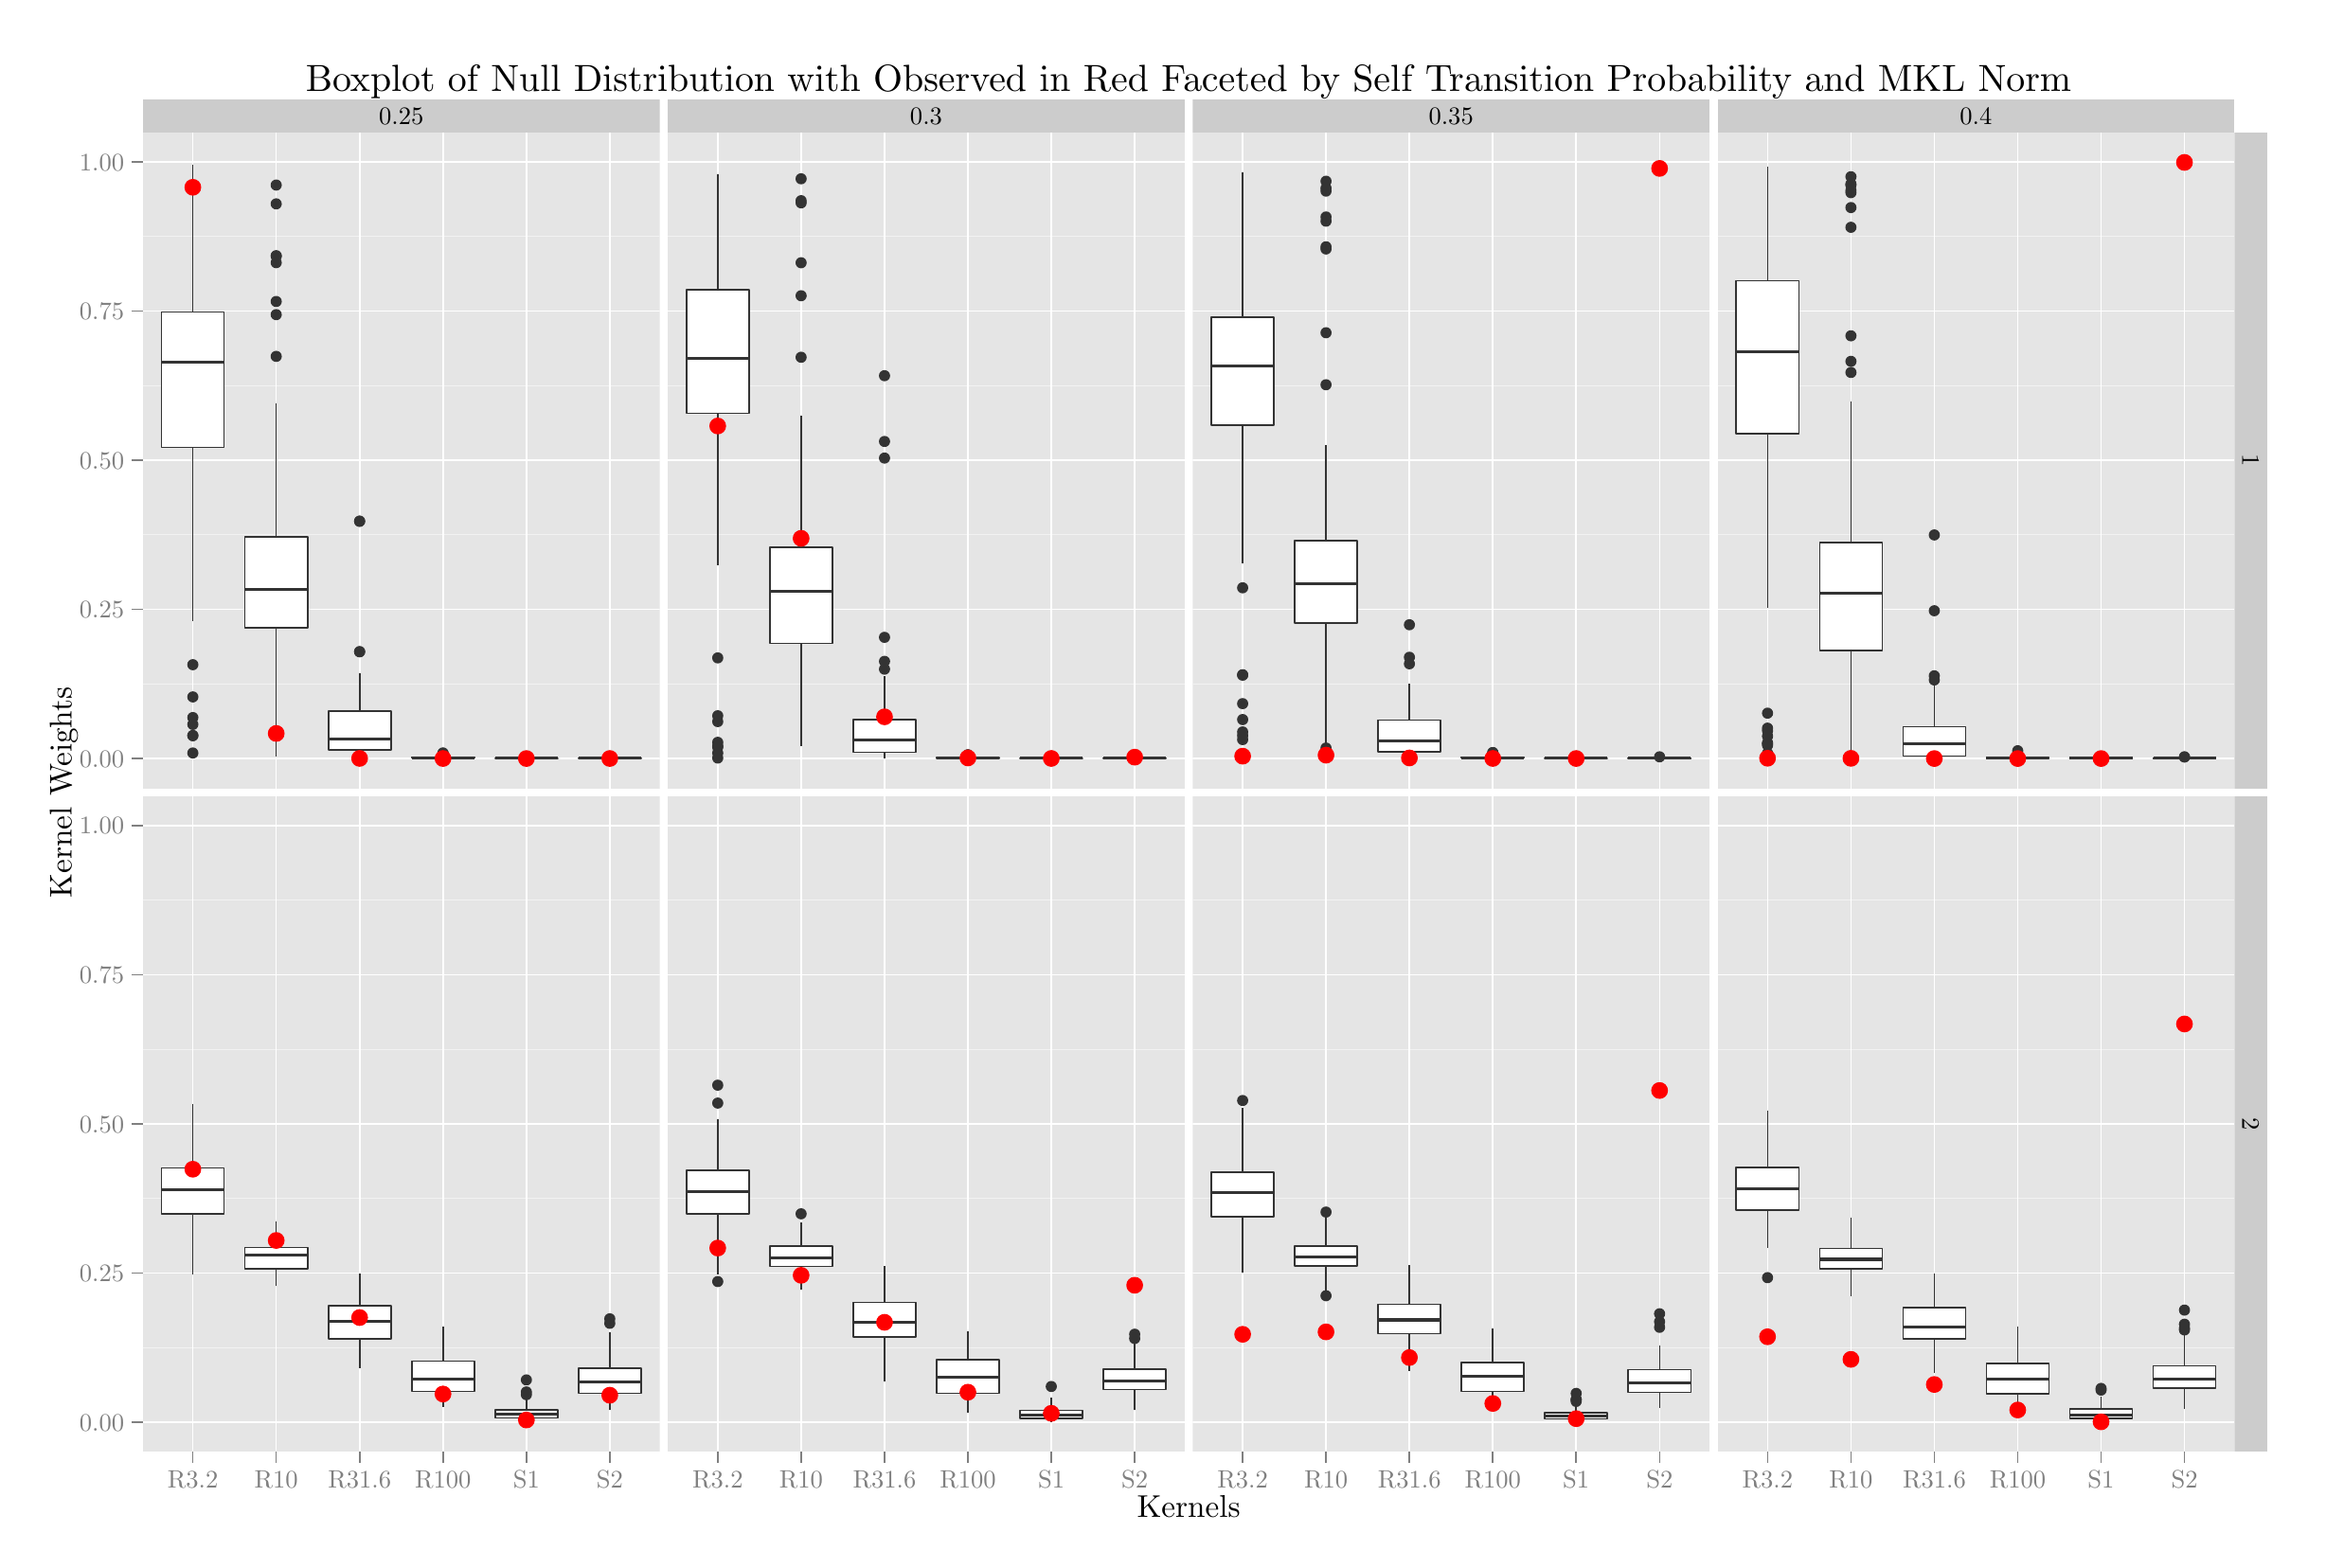
\begin{tikzpicture}[x=1pt,y=1pt]
\definecolor[named]{fillColor}{rgb}{1.00,1.00,1.00}
\path[use as bounding box,fill=fillColor,fill opacity=0.00] (0,0) rectangle (867.24,578.16);
\begin{scope}
\path[clip] (  0.00,  0.00) rectangle (867.24,578.16);
\definecolor[named]{drawColor}{rgb}{1.00,1.00,1.00}
\definecolor[named]{fillColor}{rgb}{1.00,1.00,1.00}

\path[draw=drawColor,line width= 0.6pt,line join=round,line cap=round,fill=fillColor] ( -0.00,  0.00) rectangle (867.24,578.16);
\end{scope}
\begin{scope}
\path[clip] ( 44.49,537.54) rectangle (241.75,550.17);
\definecolor[named]{fillColor}{rgb}{0.80,0.80,0.80}

\path[fill=fillColor] ( 44.49,537.54) rectangle (241.75,550.17);
\definecolor[named]{drawColor}{rgb}{0.00,0.00,0.00}

\node[text=drawColor,anchor=base,inner sep=0pt, outer sep=0pt, scale=  0.96] at (143.12,540.55) {0.25};
\end{scope}
\begin{scope}
\path[clip] (244.76,537.54) rectangle (442.02,550.17);
\definecolor[named]{fillColor}{rgb}{0.80,0.80,0.80}

\path[fill=fillColor] (244.76,537.54) rectangle (442.02,550.17);
\definecolor[named]{drawColor}{rgb}{0.00,0.00,0.00}

\node[text=drawColor,anchor=base,inner sep=0pt, outer sep=0pt, scale=  0.96] at (343.39,540.55) {0.3};
\end{scope}
\begin{scope}
\path[clip] (445.03,537.54) rectangle (642.29,550.17);
\definecolor[named]{fillColor}{rgb}{0.80,0.80,0.80}

\path[fill=fillColor] (445.03,537.54) rectangle (642.29,550.17);
\definecolor[named]{drawColor}{rgb}{0.00,0.00,0.00}

\node[text=drawColor,anchor=base,inner sep=0pt, outer sep=0pt, scale=  0.96] at (543.66,540.55) {0.35};
\end{scope}
\begin{scope}
\path[clip] (645.30,537.54) rectangle (842.56,550.17);
\definecolor[named]{fillColor}{rgb}{0.80,0.80,0.80}

\path[fill=fillColor] (645.30,537.54) rectangle (842.56,550.17);
\definecolor[named]{drawColor}{rgb}{0.00,0.00,0.00}

\node[text=drawColor,anchor=base,inner sep=0pt, outer sep=0pt, scale=  0.96] at (743.93,540.55) {0.4};
\end{scope}
\begin{scope}
\path[clip] ( 44.49,287.29) rectangle (241.75,537.54);
\definecolor[named]{fillColor}{rgb}{0.90,0.90,0.90}

\path[fill=fillColor] ( 44.49,287.29) rectangle (241.75,537.54);
\definecolor[named]{drawColor}{rgb}{0.95,0.95,0.95}

\path[draw=drawColor,line width= 0.3pt,line join=round] ( 44.49,327.13) --
	(241.75,327.13);

\path[draw=drawColor,line width= 0.3pt,line join=round] ( 44.49,384.06) --
	(241.75,384.06);

\path[draw=drawColor,line width= 0.3pt,line join=round] ( 44.49,440.99) --
	(241.75,440.99);

\path[draw=drawColor,line width= 0.3pt,line join=round] ( 44.49,497.92) --
	(241.75,497.92);
\definecolor[named]{drawColor}{rgb}{1.00,1.00,1.00}

\path[draw=drawColor,line width= 0.6pt,line join=round] ( 44.49,298.67) --
	(241.75,298.67);

\path[draw=drawColor,line width= 0.6pt,line join=round] ( 44.49,355.60) --
	(241.75,355.60);

\path[draw=drawColor,line width= 0.6pt,line join=round] ( 44.49,412.52) --
	(241.75,412.52);

\path[draw=drawColor,line width= 0.6pt,line join=round] ( 44.49,469.45) --
	(241.75,469.45);

\path[draw=drawColor,line width= 0.6pt,line join=round] ( 44.49,526.38) --
	(241.75,526.38);

\path[draw=drawColor,line width= 0.6pt,line join=round] ( 63.58,287.29) --
	( 63.58,537.54);

\path[draw=drawColor,line width= 0.6pt,line join=round] ( 95.39,287.29) --
	( 95.39,537.54);

\path[draw=drawColor,line width= 0.6pt,line join=round] (127.21,287.29) --
	(127.21,537.54);

\path[draw=drawColor,line width= 0.6pt,line join=round] (159.02,287.29) --
	(159.02,537.54);

\path[draw=drawColor,line width= 0.6pt,line join=round] (190.84,287.29) --
	(190.84,537.54);

\path[draw=drawColor,line width= 0.6pt,line join=round] (222.66,287.29) --
	(222.66,537.54);
\definecolor[named]{fillColor}{rgb}{0.20,0.20,0.20}

\path[fill=fillColor] ( 63.58,307.38) circle (  2.13);

\path[fill=fillColor] ( 63.58,314.31) circle (  2.13);

\path[fill=fillColor] ( 63.58,307.48) circle (  2.13);

\path[fill=fillColor] ( 63.58,300.79) circle (  2.13);

\path[fill=fillColor] ( 63.58,334.49) circle (  2.13);

\path[fill=fillColor] ( 63.58,311.70) circle (  2.13);

\path[fill=fillColor] ( 63.58,322.19) circle (  2.13);
\definecolor[named]{drawColor}{rgb}{0.20,0.20,0.20}

\path[draw=drawColor,line width= 0.6pt,line join=round,fill=fillColor] ( 63.58,469.10) -- ( 63.58,525.42);

\path[draw=drawColor,line width= 0.6pt,line join=round,fill=fillColor] ( 63.58,417.47) -- ( 63.58,351.27);
\definecolor[named]{fillColor}{rgb}{1.00,1.00,1.00}

\path[draw=drawColor,line width= 0.6pt,line join=round,line cap=round,fill=fillColor] ( 51.64,469.10) --
	( 51.64,417.47) --
	( 75.51,417.47) --
	( 75.51,469.10) --
	( 51.64,469.10) --
	cycle;
\definecolor[named]{fillColor}{rgb}{0.20,0.20,0.20}

\path[draw=drawColor,line width= 1.1pt,line join=round,fill=fillColor] ( 51.64,449.89) -- ( 75.51,449.89);

\path[fill=fillColor] ( 95.39,517.53) circle (  2.13);

\path[fill=fillColor] ( 95.39,510.35) circle (  2.13);

\path[fill=fillColor] ( 95.39,490.57) circle (  2.13);

\path[fill=fillColor] ( 95.39,473.10) circle (  2.13);

\path[fill=fillColor] ( 95.39,468.08) circle (  2.13);

\path[fill=fillColor] ( 95.39,490.38) circle (  2.13);

\path[fill=fillColor] ( 95.39,452.15) circle (  2.13);

\path[fill=fillColor] ( 95.39,487.91) circle (  2.13);

\path[draw=drawColor,line width= 0.6pt,line join=round,fill=fillColor] ( 95.39,383.34) -- ( 95.39,434.24);

\path[draw=drawColor,line width= 0.6pt,line join=round,fill=fillColor] ( 95.39,348.56) -- ( 95.39,299.60);
\definecolor[named]{fillColor}{rgb}{1.00,1.00,1.00}

\path[draw=drawColor,line width= 0.6pt,line join=round,line cap=round,fill=fillColor] ( 83.46,383.34) --
	( 83.46,348.56) --
	(107.32,348.56) --
	(107.32,383.34) --
	( 83.46,383.34) --
	cycle;
\definecolor[named]{fillColor}{rgb}{0.20,0.20,0.20}

\path[draw=drawColor,line width= 1.1pt,line join=round,fill=fillColor] ( 83.46,363.31) -- (107.32,363.31);

\path[fill=fillColor] (127.21,389.19) circle (  2.13);

\path[fill=fillColor] (127.21,339.46) circle (  2.13);

\path[fill=fillColor] (127.21,389.29) circle (  2.13);

\path[fill=fillColor] (127.21,339.43) circle (  2.13);

\path[draw=drawColor,line width= 0.6pt,line join=round,fill=fillColor] (127.21,316.88) -- (127.21,331.41);

\path[draw=drawColor,line width= 0.6pt,line join=round,fill=fillColor] (127.21,301.99) -- (127.21,298.68);
\definecolor[named]{fillColor}{rgb}{1.00,1.00,1.00}

\path[draw=drawColor,line width= 0.6pt,line join=round,line cap=round,fill=fillColor] (115.28,316.88) --
	(115.28,301.99) --
	(139.14,301.99) --
	(139.14,316.88) --
	(115.28,316.88) --
	cycle;
\definecolor[named]{fillColor}{rgb}{0.20,0.20,0.20}

\path[draw=drawColor,line width= 1.1pt,line join=round,fill=fillColor] (115.28,306.04) -- (139.14,306.04);

\path[fill=fillColor] (159.02,300.36) circle (  2.13);

\path[fill=fillColor] (159.02,300.29) circle (  2.13);

\path[fill=fillColor] (159.02,299.94) circle (  2.13);

\path[fill=fillColor] (159.02,300.17) circle (  2.13);

\path[fill=fillColor] (159.02,300.68) circle (  2.13);

\path[fill=fillColor] (159.02,300.80) circle (  2.13);

\path[fill=fillColor] (159.02,300.49) circle (  2.13);

\path[fill=fillColor] (159.02,299.97) circle (  2.13);

\path[fill=fillColor] (159.02,300.05) circle (  2.13);

\path[draw=drawColor,line width= 0.6pt,line join=round,fill=fillColor] (159.02,299.29) -- (159.02,299.82);

\path[draw=drawColor,line width= 0.6pt,line join=round,fill=fillColor] (159.02,298.86) -- (159.02,298.67);
\definecolor[named]{fillColor}{rgb}{1.00,1.00,1.00}

\path[draw=drawColor,line width= 0.6pt,line join=round,line cap=round,fill=fillColor] (147.09,299.29) --
	(147.09,298.86) --
	(170.95,298.86) --
	(170.95,299.29) --
	(147.09,299.29) --
	cycle;
\definecolor[named]{fillColor}{rgb}{0.20,0.20,0.20}

\path[draw=drawColor,line width= 1.1pt,line join=round,fill=fillColor] (147.09,298.99) -- (170.95,298.99);

\path[draw=drawColor,line width= 0.6pt,line join=round,fill=fillColor] (190.84,298.83) -- (190.84,298.97);

\path[draw=drawColor,line width= 0.6pt,line join=round,fill=fillColor] (190.84,298.71) -- (190.84,298.67);
\definecolor[named]{fillColor}{rgb}{1.00,1.00,1.00}

\path[draw=drawColor,line width= 0.6pt,line join=round,line cap=round,fill=fillColor] (178.91,298.83) --
	(178.91,298.71) --
	(202.77,298.71) --
	(202.77,298.83) --
	(178.91,298.83) --
	cycle;
\definecolor[named]{fillColor}{rgb}{0.20,0.20,0.20}

\path[draw=drawColor,line width= 1.1pt,line join=round,fill=fillColor] (178.91,298.78) -- (202.77,298.78);

\path[fill=fillColor] (222.66,299.26) circle (  2.13);

\path[draw=drawColor,line width= 0.6pt,line join=round,fill=fillColor] (222.66,298.94) -- (222.66,299.16);

\path[draw=drawColor,line width= 0.6pt,line join=round,fill=fillColor] (222.66,298.73) -- (222.66,298.67);
\definecolor[named]{fillColor}{rgb}{1.00,1.00,1.00}

\path[draw=drawColor,line width= 0.6pt,line join=round,line cap=round,fill=fillColor] (210.73,298.94) --
	(210.73,298.73) --
	(234.59,298.73) --
	(234.59,298.94) --
	(210.73,298.94) --
	cycle;
\definecolor[named]{fillColor}{rgb}{0.20,0.20,0.20}

\path[draw=drawColor,line width= 1.1pt,line join=round,fill=fillColor] (210.73,298.86) -- (234.59,298.86);
\definecolor[named]{fillColor}{rgb}{1.00,0.00,0.00}

\path[fill=fillColor] ( 63.58,516.68) circle (  3.20);

\path[fill=fillColor] ( 95.39,308.25) circle (  3.20);

\path[fill=fillColor] (127.21,298.73) circle (  3.20);

\path[fill=fillColor] (159.02,298.69) circle (  3.20);

\path[fill=fillColor] (190.84,298.68) circle (  3.20);

\path[fill=fillColor] (222.66,298.69) circle (  3.20);
\end{scope}
\begin{scope}
\path[clip] ( 44.49, 34.03) rectangle (241.75,284.28);
\definecolor[named]{fillColor}{rgb}{0.90,0.90,0.90}

\path[fill=fillColor] ( 44.49, 34.03) rectangle (241.75,284.28);
\definecolor[named]{drawColor}{rgb}{0.95,0.95,0.95}

\path[draw=drawColor,line width= 0.3pt,line join=round] ( 44.49, 73.87) --
	(241.75, 73.87);

\path[draw=drawColor,line width= 0.3pt,line join=round] ( 44.49,130.80) --
	(241.75,130.80);

\path[draw=drawColor,line width= 0.3pt,line join=round] ( 44.49,187.73) --
	(241.75,187.73);

\path[draw=drawColor,line width= 0.3pt,line join=round] ( 44.49,244.66) --
	(241.75,244.66);
\definecolor[named]{drawColor}{rgb}{1.00,1.00,1.00}

\path[draw=drawColor,line width= 0.6pt,line join=round] ( 44.49, 45.41) --
	(241.75, 45.41);

\path[draw=drawColor,line width= 0.6pt,line join=round] ( 44.49,102.34) --
	(241.75,102.34);

\path[draw=drawColor,line width= 0.6pt,line join=round] ( 44.49,159.26) --
	(241.75,159.26);

\path[draw=drawColor,line width= 0.6pt,line join=round] ( 44.49,216.19) --
	(241.75,216.19);

\path[draw=drawColor,line width= 0.6pt,line join=round] ( 44.49,273.12) --
	(241.75,273.12);

\path[draw=drawColor,line width= 0.6pt,line join=round] ( 63.58, 34.03) --
	( 63.58,284.28);

\path[draw=drawColor,line width= 0.6pt,line join=round] ( 95.39, 34.03) --
	( 95.39,284.28);

\path[draw=drawColor,line width= 0.6pt,line join=round] (127.21, 34.03) --
	(127.21,284.28);

\path[draw=drawColor,line width= 0.6pt,line join=round] (159.02, 34.03) --
	(159.02,284.28);

\path[draw=drawColor,line width= 0.6pt,line join=round] (190.84, 34.03) --
	(190.84,284.28);

\path[draw=drawColor,line width= 0.6pt,line join=round] (222.66, 34.03) --
	(222.66,284.28);
\definecolor[named]{drawColor}{rgb}{0.20,0.20,0.20}
\definecolor[named]{fillColor}{rgb}{0.20,0.20,0.20}

\path[draw=drawColor,line width= 0.6pt,line join=round,fill=fillColor] ( 63.58,142.43) -- ( 63.58,166.88);

\path[draw=drawColor,line width= 0.6pt,line join=round,fill=fillColor] ( 63.58,124.91) -- ( 63.58,101.89);
\definecolor[named]{fillColor}{rgb}{1.00,1.00,1.00}

\path[draw=drawColor,line width= 0.6pt,line join=round,line cap=round,fill=fillColor] ( 51.64,142.43) --
	( 51.64,124.91) --
	( 75.51,124.91) --
	( 75.51,142.43) --
	( 51.64,142.43) --
	cycle;
\definecolor[named]{fillColor}{rgb}{0.20,0.20,0.20}

\path[draw=drawColor,line width= 1.1pt,line join=round,fill=fillColor] ( 51.64,134.06) -- ( 75.51,134.06);

\path[draw=drawColor,line width= 0.6pt,line join=round,fill=fillColor] ( 95.39,112.12) -- ( 95.39,122.17);

\path[draw=drawColor,line width= 0.6pt,line join=round,fill=fillColor] ( 95.39,104.05) -- ( 95.39, 97.30);
\definecolor[named]{fillColor}{rgb}{1.00,1.00,1.00}

\path[draw=drawColor,line width= 0.6pt,line join=round,line cap=round,fill=fillColor] ( 83.46,112.12) --
	( 83.46,104.05) --
	(107.32,104.05) --
	(107.32,112.12) --
	( 83.46,112.12) --
	cycle;
\definecolor[named]{fillColor}{rgb}{0.20,0.20,0.20}

\path[draw=drawColor,line width= 1.1pt,line join=round,fill=fillColor] ( 83.46,109.03) -- (107.32,109.03);

\path[draw=drawColor,line width= 0.6pt,line join=round,fill=fillColor] (127.21, 89.76) -- (127.21,101.99);

\path[draw=drawColor,line width= 0.6pt,line join=round,fill=fillColor] (127.21, 77.13) -- (127.21, 66.07);
\definecolor[named]{fillColor}{rgb}{1.00,1.00,1.00}

\path[draw=drawColor,line width= 0.6pt,line join=round,line cap=round,fill=fillColor] (115.28, 89.76) --
	(115.28, 77.13) --
	(139.14, 77.13) --
	(139.14, 89.76) --
	(115.28, 89.76) --
	cycle;
\definecolor[named]{fillColor}{rgb}{0.20,0.20,0.20}

\path[draw=drawColor,line width= 1.1pt,line join=round,fill=fillColor] (115.28, 83.75) -- (139.14, 83.75);

\path[draw=drawColor,line width= 0.6pt,line join=round,fill=fillColor] (159.02, 68.66) -- (159.02, 81.78);

\path[draw=drawColor,line width= 0.6pt,line join=round,fill=fillColor] (159.02, 57.13) -- (159.02, 51.25);
\definecolor[named]{fillColor}{rgb}{1.00,1.00,1.00}

\path[draw=drawColor,line width= 0.6pt,line join=round,line cap=round,fill=fillColor] (147.09, 68.66) --
	(147.09, 57.13) --
	(170.95, 57.13) --
	(170.95, 68.66) --
	(147.09, 68.66) --
	cycle;
\definecolor[named]{fillColor}{rgb}{0.20,0.20,0.20}

\path[draw=drawColor,line width= 1.1pt,line join=round,fill=fillColor] (147.09, 61.99) -- (170.95, 61.99);

\path[fill=fillColor] (190.84, 55.91) circle (  2.13);

\path[fill=fillColor] (190.84, 61.55) circle (  2.13);

\path[fill=fillColor] (190.84, 56.96) circle (  2.13);

\path[draw=drawColor,line width= 0.6pt,line join=round,fill=fillColor] (190.84, 50.14) -- (190.84, 54.71);

\path[draw=drawColor,line width= 0.6pt,line join=round,fill=fillColor] (190.84, 47.08) -- (190.84, 45.57);
\definecolor[named]{fillColor}{rgb}{1.00,1.00,1.00}

\path[draw=drawColor,line width= 0.6pt,line join=round,line cap=round,fill=fillColor] (178.91, 50.14) --
	(178.91, 47.08) --
	(202.77, 47.08) --
	(202.77, 50.14) --
	(178.91, 50.14) --
	cycle;
\definecolor[named]{fillColor}{rgb}{0.20,0.20,0.20}

\path[draw=drawColor,line width= 1.1pt,line join=round,fill=fillColor] (178.91, 48.41) -- (202.77, 48.41);

\path[fill=fillColor] (222.66, 84.85) circle (  2.13);

\path[fill=fillColor] (222.66, 83.13) circle (  2.13);

\path[draw=drawColor,line width= 0.6pt,line join=round,fill=fillColor] (222.66, 65.95) -- (222.66, 79.86);

\path[draw=drawColor,line width= 0.6pt,line join=round,fill=fillColor] (222.66, 56.46) -- (222.66, 49.93);
\definecolor[named]{fillColor}{rgb}{1.00,1.00,1.00}

\path[draw=drawColor,line width= 0.6pt,line join=round,line cap=round,fill=fillColor] (210.73, 65.95) --
	(210.73, 56.46) --
	(234.59, 56.46) --
	(234.59, 65.95) --
	(210.73, 65.95) --
	cycle;
\definecolor[named]{fillColor}{rgb}{0.20,0.20,0.20}

\path[draw=drawColor,line width= 1.1pt,line join=round,fill=fillColor] (210.73, 60.61) -- (234.59, 60.61);
\definecolor[named]{fillColor}{rgb}{1.00,0.00,0.00}

\path[fill=fillColor] ( 63.58,141.95) circle (  3.20);

\path[fill=fillColor] ( 95.39,114.76) circle (  3.20);

\path[fill=fillColor] (127.21, 85.34) circle (  3.20);

\path[fill=fillColor] (159.02, 56.16) circle (  3.20);

\path[fill=fillColor] (190.84, 46.25) circle (  3.20);

\path[fill=fillColor] (222.66, 55.70) circle (  3.20);
\end{scope}
\begin{scope}
\path[clip] (244.76,287.29) rectangle (442.02,537.54);
\definecolor[named]{fillColor}{rgb}{0.90,0.90,0.90}

\path[fill=fillColor] (244.76,287.29) rectangle (442.02,537.54);
\definecolor[named]{drawColor}{rgb}{0.95,0.95,0.95}

\path[draw=drawColor,line width= 0.3pt,line join=round] (244.76,327.13) --
	(442.02,327.13);

\path[draw=drawColor,line width= 0.3pt,line join=round] (244.76,384.06) --
	(442.02,384.06);

\path[draw=drawColor,line width= 0.3pt,line join=round] (244.76,440.99) --
	(442.02,440.99);

\path[draw=drawColor,line width= 0.3pt,line join=round] (244.76,497.92) --
	(442.02,497.92);
\definecolor[named]{drawColor}{rgb}{1.00,1.00,1.00}

\path[draw=drawColor,line width= 0.6pt,line join=round] (244.76,298.67) --
	(442.02,298.67);

\path[draw=drawColor,line width= 0.6pt,line join=round] (244.76,355.60) --
	(442.02,355.60);

\path[draw=drawColor,line width= 0.6pt,line join=round] (244.76,412.52) --
	(442.02,412.52);

\path[draw=drawColor,line width= 0.6pt,line join=round] (244.76,469.45) --
	(442.02,469.45);

\path[draw=drawColor,line width= 0.6pt,line join=round] (244.76,526.38) --
	(442.02,526.38);

\path[draw=drawColor,line width= 0.6pt,line join=round] (263.85,287.29) --
	(263.85,537.54);

\path[draw=drawColor,line width= 0.6pt,line join=round] (295.66,287.29) --
	(295.66,537.54);

\path[draw=drawColor,line width= 0.6pt,line join=round] (327.48,287.29) --
	(327.48,537.54);

\path[draw=drawColor,line width= 0.6pt,line join=round] (359.30,287.29) --
	(359.30,537.54);

\path[draw=drawColor,line width= 0.6pt,line join=round] (391.11,287.29) --
	(391.11,537.54);

\path[draw=drawColor,line width= 0.6pt,line join=round] (422.93,287.29) --
	(422.93,537.54);
\definecolor[named]{fillColor}{rgb}{0.20,0.20,0.20}

\path[fill=fillColor] (263.85,312.78) circle (  2.13);

\path[fill=fillColor] (263.85,303.05) circle (  2.13);

\path[fill=fillColor] (263.85,298.86) circle (  2.13);

\path[fill=fillColor] (263.85,315.00) circle (  2.13);

\path[fill=fillColor] (263.85,300.79) circle (  2.13);

\path[fill=fillColor] (263.85,304.86) circle (  2.13);

\path[fill=fillColor] (263.85,337.08) circle (  2.13);

\path[fill=fillColor] (263.85,303.44) circle (  2.13);
\definecolor[named]{drawColor}{rgb}{0.20,0.20,0.20}

\path[draw=drawColor,line width= 0.6pt,line join=round,fill=fillColor] (263.85,477.54) -- (263.85,521.61);

\path[draw=drawColor,line width= 0.6pt,line join=round,fill=fillColor] (263.85,430.46) -- (263.85,372.39);
\definecolor[named]{fillColor}{rgb}{1.00,1.00,1.00}

\path[draw=drawColor,line width= 0.6pt,line join=round,line cap=round,fill=fillColor] (251.92,477.54) --
	(251.92,430.46) --
	(275.78,430.46) --
	(275.78,477.54) --
	(251.92,477.54) --
	cycle;
\definecolor[named]{fillColor}{rgb}{0.20,0.20,0.20}

\path[draw=drawColor,line width= 1.1pt,line join=round,fill=fillColor] (251.92,451.30) -- (275.78,451.30);

\path[fill=fillColor] (295.66,511.56) circle (  2.13);

\path[fill=fillColor] (295.66,451.82) circle (  2.13);

\path[fill=fillColor] (295.66,510.74) circle (  2.13);

\path[fill=fillColor] (295.66,519.92) circle (  2.13);

\path[fill=fillColor] (295.66,487.88) circle (  2.13);

\path[fill=fillColor] (295.66,475.29) circle (  2.13);

\path[draw=drawColor,line width= 0.6pt,line join=round,fill=fillColor] (295.66,379.19) -- (295.66,429.63);

\path[draw=drawColor,line width= 0.6pt,line join=round,fill=fillColor] (295.66,342.57) -- (295.66,303.36);
\definecolor[named]{fillColor}{rgb}{1.00,1.00,1.00}

\path[draw=drawColor,line width= 0.6pt,line join=round,line cap=round,fill=fillColor] (283.73,379.19) --
	(283.73,342.57) --
	(307.59,342.57) --
	(307.59,379.19) --
	(283.73,379.19) --
	cycle;
\definecolor[named]{fillColor}{rgb}{0.20,0.20,0.20}

\path[draw=drawColor,line width= 1.1pt,line join=round,fill=fillColor] (283.73,362.49) -- (307.59,362.49);

\path[fill=fillColor] (327.48,335.76) circle (  2.13);

\path[fill=fillColor] (327.48,444.77) circle (  2.13);

\path[fill=fillColor] (327.48,332.78) circle (  2.13);

\path[fill=fillColor] (327.48,419.68) circle (  2.13);

\path[fill=fillColor] (327.48,413.34) circle (  2.13);

\path[fill=fillColor] (327.48,344.93) circle (  2.13);

\path[draw=drawColor,line width= 0.6pt,line join=round,fill=fillColor] (327.48,313.54) -- (327.48,330.05);

\path[draw=drawColor,line width= 0.6pt,line join=round,fill=fillColor] (327.48,301.08) -- (327.48,298.70);
\definecolor[named]{fillColor}{rgb}{1.00,1.00,1.00}

\path[draw=drawColor,line width= 0.6pt,line join=round,line cap=round,fill=fillColor] (315.55,313.54) --
	(315.55,301.08) --
	(339.41,301.08) --
	(339.41,313.54) --
	(315.55,313.54) --
	cycle;
\definecolor[named]{fillColor}{rgb}{0.20,0.20,0.20}

\path[draw=drawColor,line width= 1.1pt,line join=round,fill=fillColor] (315.55,305.87) -- (339.41,305.87);

\path[fill=fillColor] (359.30,300.05) circle (  2.13);

\path[fill=fillColor] (359.30,300.11) circle (  2.13);

\path[fill=fillColor] (359.30,299.86) circle (  2.13);

\path[fill=fillColor] (359.30,299.72) circle (  2.13);

\path[fill=fillColor] (359.30,299.80) circle (  2.13);

\path[fill=fillColor] (359.30,299.71) circle (  2.13);

\path[draw=drawColor,line width= 0.6pt,line join=round,fill=fillColor] (359.30,299.16) -- (359.30,299.67);

\path[draw=drawColor,line width= 0.6pt,line join=round,fill=fillColor] (359.30,298.81) -- (359.30,298.68);
\definecolor[named]{fillColor}{rgb}{1.00,1.00,1.00}

\path[draw=drawColor,line width= 0.6pt,line join=round,line cap=round,fill=fillColor] (347.36,299.16) --
	(347.36,298.81) --
	(371.23,298.81) --
	(371.23,299.16) --
	(347.36,299.16) --
	cycle;
\definecolor[named]{fillColor}{rgb}{0.20,0.20,0.20}

\path[draw=drawColor,line width= 1.1pt,line join=round,fill=fillColor] (347.36,298.96) -- (371.23,298.96);

\path[fill=fillColor] (391.11,299.17) circle (  2.13);

\path[fill=fillColor] (391.11,299.08) circle (  2.13);

\path[draw=drawColor,line width= 0.6pt,line join=round,fill=fillColor] (391.11,298.82) -- (391.11,298.97);

\path[draw=drawColor,line width= 0.6pt,line join=round,fill=fillColor] (391.11,298.71) -- (391.11,298.67);
\definecolor[named]{fillColor}{rgb}{1.00,1.00,1.00}

\path[draw=drawColor,line width= 0.6pt,line join=round,line cap=round,fill=fillColor] (379.18,298.82) --
	(379.18,298.71) --
	(403.04,298.71) --
	(403.04,298.82) --
	(379.18,298.82) --
	cycle;
\definecolor[named]{fillColor}{rgb}{0.20,0.20,0.20}

\path[draw=drawColor,line width= 1.1pt,line join=round,fill=fillColor] (379.18,298.77) -- (403.04,298.77);

\path[fill=fillColor] (422.93,299.90) circle (  2.13);

\path[fill=fillColor] (422.93,299.36) circle (  2.13);

\path[fill=fillColor] (422.93,299.32) circle (  2.13);

\path[fill=fillColor] (422.93,299.61) circle (  2.13);

\path[draw=drawColor,line width= 0.6pt,line join=round,fill=fillColor] (422.93,298.90) -- (422.93,299.07);

\path[draw=drawColor,line width= 0.6pt,line join=round,fill=fillColor] (422.93,298.74) -- (422.93,298.67);
\definecolor[named]{fillColor}{rgb}{1.00,1.00,1.00}

\path[draw=drawColor,line width= 0.6pt,line join=round,line cap=round,fill=fillColor] (411.00,298.90) --
	(411.00,298.74) --
	(434.86,298.74) --
	(434.86,298.90) --
	(411.00,298.90) --
	cycle;
\definecolor[named]{fillColor}{rgb}{0.20,0.20,0.20}

\path[draw=drawColor,line width= 1.1pt,line join=round,fill=fillColor] (411.00,298.84) -- (434.86,298.84);
\definecolor[named]{fillColor}{rgb}{1.00,0.00,0.00}

\path[fill=fillColor] (263.85,425.59) circle (  3.20);

\path[fill=fillColor] (295.66,382.71) circle (  3.20);

\path[fill=fillColor] (327.48,314.59) circle (  3.20);

\path[fill=fillColor] (359.30,298.91) circle (  3.20);

\path[fill=fillColor] (391.11,298.71) circle (  3.20);

\path[fill=fillColor] (422.93,299.20) circle (  3.20);
\end{scope}
\begin{scope}
\path[clip] (244.76, 34.03) rectangle (442.02,284.28);
\definecolor[named]{fillColor}{rgb}{0.90,0.90,0.90}

\path[fill=fillColor] (244.76, 34.03) rectangle (442.02,284.28);
\definecolor[named]{drawColor}{rgb}{0.95,0.95,0.95}

\path[draw=drawColor,line width= 0.3pt,line join=round] (244.76, 73.87) --
	(442.02, 73.87);

\path[draw=drawColor,line width= 0.3pt,line join=round] (244.76,130.80) --
	(442.02,130.80);

\path[draw=drawColor,line width= 0.3pt,line join=round] (244.76,187.73) --
	(442.02,187.73);

\path[draw=drawColor,line width= 0.3pt,line join=round] (244.76,244.66) --
	(442.02,244.66);
\definecolor[named]{drawColor}{rgb}{1.00,1.00,1.00}

\path[draw=drawColor,line width= 0.6pt,line join=round] (244.76, 45.41) --
	(442.02, 45.41);

\path[draw=drawColor,line width= 0.6pt,line join=round] (244.76,102.34) --
	(442.02,102.34);

\path[draw=drawColor,line width= 0.6pt,line join=round] (244.76,159.26) --
	(442.02,159.26);

\path[draw=drawColor,line width= 0.6pt,line join=round] (244.76,216.19) --
	(442.02,216.19);

\path[draw=drawColor,line width= 0.6pt,line join=round] (244.76,273.12) --
	(442.02,273.12);

\path[draw=drawColor,line width= 0.6pt,line join=round] (263.85, 34.03) --
	(263.85,284.28);

\path[draw=drawColor,line width= 0.6pt,line join=round] (295.66, 34.03) --
	(295.66,284.28);

\path[draw=drawColor,line width= 0.6pt,line join=round] (327.48, 34.03) --
	(327.48,284.28);

\path[draw=drawColor,line width= 0.6pt,line join=round] (359.30, 34.03) --
	(359.30,284.28);

\path[draw=drawColor,line width= 0.6pt,line join=round] (391.11, 34.03) --
	(391.11,284.28);

\path[draw=drawColor,line width= 0.6pt,line join=round] (422.93, 34.03) --
	(422.93,284.28);
\definecolor[named]{fillColor}{rgb}{0.20,0.20,0.20}

\path[fill=fillColor] (263.85,174.02) circle (  2.13);

\path[fill=fillColor] (263.85,167.19) circle (  2.13);

\path[fill=fillColor] (263.85, 99.08) circle (  2.13);
\definecolor[named]{drawColor}{rgb}{0.20,0.20,0.20}

\path[draw=drawColor,line width= 0.6pt,line join=round,fill=fillColor] (263.85,141.42) -- (263.85,161.04);

\path[draw=drawColor,line width= 0.6pt,line join=round,fill=fillColor] (263.85,125.00) -- (263.85,101.89);
\definecolor[named]{fillColor}{rgb}{1.00,1.00,1.00}

\path[draw=drawColor,line width= 0.6pt,line join=round,line cap=round,fill=fillColor] (251.92,141.42) --
	(251.92,125.00) --
	(275.78,125.00) --
	(275.78,141.42) --
	(251.92,141.42) --
	cycle;
\definecolor[named]{fillColor}{rgb}{0.20,0.20,0.20}

\path[draw=drawColor,line width= 1.1pt,line join=round,fill=fillColor] (251.92,133.50) -- (275.78,133.50);

\path[fill=fillColor] (295.66,124.93) circle (  2.13);

\path[draw=drawColor,line width= 0.6pt,line join=round,fill=fillColor] (295.66,112.62) -- (295.66,121.75);

\path[draw=drawColor,line width= 0.6pt,line join=round,fill=fillColor] (295.66,104.82) -- (295.66, 95.83);
\definecolor[named]{fillColor}{rgb}{1.00,1.00,1.00}

\path[draw=drawColor,line width= 0.6pt,line join=round,line cap=round,fill=fillColor] (283.73,112.62) --
	(283.73,104.82) --
	(307.59,104.82) --
	(307.59,112.62) --
	(283.73,112.62) --
	cycle;
\definecolor[named]{fillColor}{rgb}{0.20,0.20,0.20}

\path[draw=drawColor,line width= 1.1pt,line join=round,fill=fillColor] (283.73,108.02) -- (307.59,108.02);

\path[draw=drawColor,line width= 0.6pt,line join=round,fill=fillColor] (327.48, 91.06) -- (327.48,104.98);

\path[draw=drawColor,line width= 0.6pt,line join=round,fill=fillColor] (327.48, 77.82) -- (327.48, 61.03);
\definecolor[named]{fillColor}{rgb}{1.00,1.00,1.00}

\path[draw=drawColor,line width= 0.6pt,line join=round,line cap=round,fill=fillColor] (315.55, 91.06) --
	(315.55, 77.82) --
	(339.41, 77.82) --
	(339.41, 91.06) --
	(315.55, 91.06) --
	cycle;
\definecolor[named]{fillColor}{rgb}{0.20,0.20,0.20}

\path[draw=drawColor,line width= 1.1pt,line join=round,fill=fillColor] (315.55, 83.58) -- (339.41, 83.58);

\path[draw=drawColor,line width= 0.6pt,line join=round,fill=fillColor] (359.30, 69.18) -- (359.30, 80.17);

\path[draw=drawColor,line width= 0.6pt,line join=round,fill=fillColor] (359.30, 56.38) -- (359.30, 48.93);
\definecolor[named]{fillColor}{rgb}{1.00,1.00,1.00}

\path[draw=drawColor,line width= 0.6pt,line join=round,line cap=round,fill=fillColor] (347.36, 69.18) --
	(347.36, 56.38) --
	(371.23, 56.38) --
	(371.23, 69.18) --
	(347.36, 69.18) --
	cycle;
\definecolor[named]{fillColor}{rgb}{0.20,0.20,0.20}

\path[draw=drawColor,line width= 1.1pt,line join=round,fill=fillColor] (347.36, 62.45) -- (371.23, 62.45);

\path[fill=fillColor] (391.11, 59.03) circle (  2.13);

\path[draw=drawColor,line width= 0.6pt,line join=round,fill=fillColor] (391.11, 49.97) -- (391.11, 54.75);

\path[draw=drawColor,line width= 0.6pt,line join=round,fill=fillColor] (391.11, 46.78) -- (391.11, 45.54);
\definecolor[named]{fillColor}{rgb}{1.00,1.00,1.00}

\path[draw=drawColor,line width= 0.6pt,line join=round,line cap=round,fill=fillColor] (379.18, 49.97) --
	(379.18, 46.78) --
	(403.04, 46.78) --
	(403.04, 49.97) --
	(379.18, 49.97) --
	cycle;
\definecolor[named]{fillColor}{rgb}{0.20,0.20,0.20}

\path[draw=drawColor,line width= 1.1pt,line join=round,fill=fillColor] (379.18, 48.23) -- (403.04, 48.23);

\path[fill=fillColor] (422.93, 77.34) circle (  2.13);

\path[fill=fillColor] (422.93, 78.99) circle (  2.13);

\path[draw=drawColor,line width= 0.6pt,line join=round,fill=fillColor] (422.93, 65.57) -- (422.93, 76.98);

\path[draw=drawColor,line width= 0.6pt,line join=round,fill=fillColor] (422.93, 57.90) -- (422.93, 50.19);
\definecolor[named]{fillColor}{rgb}{1.00,1.00,1.00}

\path[draw=drawColor,line width= 0.6pt,line join=round,line cap=round,fill=fillColor] (411.00, 65.57) --
	(411.00, 57.90) --
	(434.86, 57.90) --
	(434.86, 65.57) --
	(411.00, 65.57) --
	cycle;
\definecolor[named]{fillColor}{rgb}{0.20,0.20,0.20}

\path[draw=drawColor,line width= 1.1pt,line join=round,fill=fillColor] (411.00, 61.22) -- (434.86, 61.22);
\definecolor[named]{fillColor}{rgb}{1.00,0.00,0.00}

\path[fill=fillColor] (263.85,111.87) circle (  3.20);

\path[fill=fillColor] (295.66,101.46) circle (  3.20);

\path[fill=fillColor] (327.48, 83.52) circle (  3.20);

\path[fill=fillColor] (359.30, 56.85) circle (  3.20);

\path[fill=fillColor] (391.11, 48.79) circle (  3.20);

\path[fill=fillColor] (422.93, 97.67) circle (  3.20);
\end{scope}
\begin{scope}
\path[clip] (445.03,287.29) rectangle (642.29,537.54);
\definecolor[named]{fillColor}{rgb}{0.90,0.90,0.90}

\path[fill=fillColor] (445.03,287.29) rectangle (642.29,537.54);
\definecolor[named]{drawColor}{rgb}{0.95,0.95,0.95}

\path[draw=drawColor,line width= 0.3pt,line join=round] (445.03,327.13) --
	(642.29,327.13);

\path[draw=drawColor,line width= 0.3pt,line join=round] (445.03,384.06) --
	(642.29,384.06);

\path[draw=drawColor,line width= 0.3pt,line join=round] (445.03,440.99) --
	(642.29,440.99);

\path[draw=drawColor,line width= 0.3pt,line join=round] (445.03,497.92) --
	(642.29,497.92);
\definecolor[named]{drawColor}{rgb}{1.00,1.00,1.00}

\path[draw=drawColor,line width= 0.6pt,line join=round] (445.03,298.67) --
	(642.29,298.67);

\path[draw=drawColor,line width= 0.6pt,line join=round] (445.03,355.60) --
	(642.29,355.60);

\path[draw=drawColor,line width= 0.6pt,line join=round] (445.03,412.52) --
	(642.29,412.52);

\path[draw=drawColor,line width= 0.6pt,line join=round] (445.03,469.45) --
	(642.29,469.45);

\path[draw=drawColor,line width= 0.6pt,line join=round] (445.03,526.38) --
	(642.29,526.38);

\path[draw=drawColor,line width= 0.6pt,line join=round] (464.12,287.29) --
	(464.12,537.54);

\path[draw=drawColor,line width= 0.6pt,line join=round] (495.93,287.29) --
	(495.93,537.54);

\path[draw=drawColor,line width= 0.6pt,line join=round] (527.75,287.29) --
	(527.75,537.54);

\path[draw=drawColor,line width= 0.6pt,line join=round] (559.57,287.29) --
	(559.57,537.54);

\path[draw=drawColor,line width= 0.6pt,line join=round] (591.38,287.29) --
	(591.38,537.54);

\path[draw=drawColor,line width= 0.6pt,line join=round] (623.20,287.29) --
	(623.20,537.54);
\definecolor[named]{fillColor}{rgb}{0.20,0.20,0.20}

\path[fill=fillColor] (464.12,313.55) circle (  2.13);

\path[fill=fillColor] (464.12,305.91) circle (  2.13);

\path[fill=fillColor] (464.12,307.44) circle (  2.13);

\path[fill=fillColor] (464.12,330.66) circle (  2.13);

\path[fill=fillColor] (464.12,363.83) circle (  2.13);

\path[fill=fillColor] (464.12,330.49) circle (  2.13);

\path[fill=fillColor] (464.12,319.63) circle (  2.13);

\path[fill=fillColor] (464.12,308.84) circle (  2.13);
\definecolor[named]{drawColor}{rgb}{0.20,0.20,0.20}

\path[draw=drawColor,line width= 0.6pt,line join=round,fill=fillColor] (464.12,467.04) -- (464.12,522.31);

\path[draw=drawColor,line width= 0.6pt,line join=round,fill=fillColor] (464.12,425.93) -- (464.12,373.24);
\definecolor[named]{fillColor}{rgb}{1.00,1.00,1.00}

\path[draw=drawColor,line width= 0.6pt,line join=round,line cap=round,fill=fillColor] (452.19,467.04) --
	(452.19,425.93) --
	(476.05,425.93) --
	(476.05,467.04) --
	(452.19,467.04) --
	cycle;
\definecolor[named]{fillColor}{rgb}{0.20,0.20,0.20}

\path[draw=drawColor,line width= 1.1pt,line join=round,fill=fillColor] (452.19,448.59) -- (476.05,448.59);

\path[fill=fillColor] (495.93,503.74) circle (  2.13);

\path[fill=fillColor] (495.93,519.00) circle (  2.13);

\path[fill=fillColor] (495.93,516.34) circle (  2.13);

\path[fill=fillColor] (495.93,302.68) circle (  2.13);

\path[fill=fillColor] (495.93,493.14) circle (  2.13);

\path[fill=fillColor] (495.93,461.18) circle (  2.13);

\path[fill=fillColor] (495.93,441.32) circle (  2.13);

\path[fill=fillColor] (495.93,493.96) circle (  2.13);

\path[fill=fillColor] (495.93,505.36) circle (  2.13);

\path[fill=fillColor] (495.93,515.22) circle (  2.13);

\path[draw=drawColor,line width= 0.6pt,line join=round,fill=fillColor] (495.93,381.71) -- (495.93,418.31);

\path[draw=drawColor,line width= 0.6pt,line join=round,fill=fillColor] (495.93,350.49) -- (495.93,303.69);
\definecolor[named]{fillColor}{rgb}{1.00,1.00,1.00}

\path[draw=drawColor,line width= 0.6pt,line join=round,line cap=round,fill=fillColor] (484.00,381.71) --
	(484.00,350.49) --
	(507.87,350.49) --
	(507.87,381.71) --
	(484.00,381.71) --
	cycle;
\definecolor[named]{fillColor}{rgb}{0.20,0.20,0.20}

\path[draw=drawColor,line width= 1.1pt,line join=round,fill=fillColor] (484.00,365.46) -- (507.87,365.46);

\path[fill=fillColor] (527.75,349.73) circle (  2.13);

\path[fill=fillColor] (527.75,334.83) circle (  2.13);

\path[fill=fillColor] (527.75,337.33) circle (  2.13);

\path[draw=drawColor,line width= 0.6pt,line join=round,fill=fillColor] (527.75,313.40) -- (527.75,327.13);

\path[draw=drawColor,line width= 0.6pt,line join=round,fill=fillColor] (527.75,301.22) -- (527.75,298.69);
\definecolor[named]{fillColor}{rgb}{1.00,1.00,1.00}

\path[draw=drawColor,line width= 0.6pt,line join=round,line cap=round,fill=fillColor] (515.82,313.40) --
	(515.82,301.22) --
	(539.68,301.22) --
	(539.68,313.40) --
	(515.82,313.40) --
	cycle;
\definecolor[named]{fillColor}{rgb}{0.20,0.20,0.20}

\path[draw=drawColor,line width= 1.1pt,line join=round,fill=fillColor] (515.82,305.49) -- (539.68,305.49);

\path[fill=fillColor] (559.57,299.99) circle (  2.13);

\path[fill=fillColor] (559.57,300.96) circle (  2.13);

\path[fill=fillColor] (559.57,300.90) circle (  2.13);

\path[fill=fillColor] (559.57,299.85) circle (  2.13);

\path[fill=fillColor] (559.57,300.60) circle (  2.13);

\path[draw=drawColor,line width= 0.6pt,line join=round,fill=fillColor] (559.57,299.22) -- (559.57,299.79);

\path[draw=drawColor,line width= 0.6pt,line join=round,fill=fillColor] (559.57,298.84) -- (559.57,298.67);
\definecolor[named]{fillColor}{rgb}{1.00,1.00,1.00}

\path[draw=drawColor,line width= 0.6pt,line join=round,line cap=round,fill=fillColor] (547.64,299.22) --
	(547.64,298.84) --
	(571.50,298.84) --
	(571.50,299.22) --
	(547.64,299.22) --
	cycle;
\definecolor[named]{fillColor}{rgb}{0.20,0.20,0.20}

\path[draw=drawColor,line width= 1.1pt,line join=round,fill=fillColor] (547.64,298.99) -- (571.50,298.99);

\path[fill=fillColor] (591.38,299.08) circle (  2.13);

\path[draw=drawColor,line width= 0.6pt,line join=round,fill=fillColor] (591.38,298.82) -- (591.38,298.97);

\path[draw=drawColor,line width= 0.6pt,line join=round,fill=fillColor] (591.38,298.71) -- (591.38,298.67);
\definecolor[named]{fillColor}{rgb}{1.00,1.00,1.00}

\path[draw=drawColor,line width= 0.6pt,line join=round,line cap=round,fill=fillColor] (579.45,298.82) --
	(579.45,298.71) --
	(603.31,298.71) --
	(603.31,298.82) --
	(579.45,298.82) --
	cycle;
\definecolor[named]{fillColor}{rgb}{0.20,0.20,0.20}

\path[draw=drawColor,line width= 1.1pt,line join=round,fill=fillColor] (579.45,298.78) -- (603.31,298.78);

\path[fill=fillColor] (623.20,299.33) circle (  2.13);

\path[draw=drawColor,line width= 0.6pt,line join=round,fill=fillColor] (623.20,298.92) -- (623.20,299.11);

\path[draw=drawColor,line width= 0.6pt,line join=round,fill=fillColor] (623.20,298.74) -- (623.20,298.67);
\definecolor[named]{fillColor}{rgb}{1.00,1.00,1.00}

\path[draw=drawColor,line width= 0.6pt,line join=round,line cap=round,fill=fillColor] (611.27,298.92) --
	(611.27,298.74) --
	(635.13,298.74) --
	(635.13,298.92) --
	(611.27,298.92) --
	cycle;
\definecolor[named]{fillColor}{rgb}{0.20,0.20,0.20}

\path[draw=drawColor,line width= 1.1pt,line join=round,fill=fillColor] (611.27,298.83) -- (635.13,298.83);
\definecolor[named]{fillColor}{rgb}{1.00,0.00,0.00}

\path[fill=fillColor] (464.12,299.58) circle (  3.20);

\path[fill=fillColor] (495.93,299.97) circle (  3.20);

\path[fill=fillColor] (527.75,298.90) circle (  3.20);

\path[fill=fillColor] (559.57,298.70) circle (  3.20);

\path[fill=fillColor] (591.38,298.69) circle (  3.20);

\path[fill=fillColor] (623.20,523.88) circle (  3.20);
\end{scope}
\begin{scope}
\path[clip] (445.03, 34.03) rectangle (642.29,284.28);
\definecolor[named]{fillColor}{rgb}{0.90,0.90,0.90}

\path[fill=fillColor] (445.03, 34.03) rectangle (642.29,284.28);
\definecolor[named]{drawColor}{rgb}{0.95,0.95,0.95}

\path[draw=drawColor,line width= 0.3pt,line join=round] (445.03, 73.87) --
	(642.29, 73.87);

\path[draw=drawColor,line width= 0.3pt,line join=round] (445.03,130.80) --
	(642.29,130.80);

\path[draw=drawColor,line width= 0.3pt,line join=round] (445.03,187.73) --
	(642.29,187.73);

\path[draw=drawColor,line width= 0.3pt,line join=round] (445.03,244.66) --
	(642.29,244.66);
\definecolor[named]{drawColor}{rgb}{1.00,1.00,1.00}

\path[draw=drawColor,line width= 0.6pt,line join=round] (445.03, 45.41) --
	(642.29, 45.41);

\path[draw=drawColor,line width= 0.6pt,line join=round] (445.03,102.34) --
	(642.29,102.34);

\path[draw=drawColor,line width= 0.6pt,line join=round] (445.03,159.26) --
	(642.29,159.26);

\path[draw=drawColor,line width= 0.6pt,line join=round] (445.03,216.19) --
	(642.29,216.19);

\path[draw=drawColor,line width= 0.6pt,line join=round] (445.03,273.12) --
	(642.29,273.12);

\path[draw=drawColor,line width= 0.6pt,line join=round] (464.12, 34.03) --
	(464.12,284.28);

\path[draw=drawColor,line width= 0.6pt,line join=round] (495.93, 34.03) --
	(495.93,284.28);

\path[draw=drawColor,line width= 0.6pt,line join=round] (527.75, 34.03) --
	(527.75,284.28);

\path[draw=drawColor,line width= 0.6pt,line join=round] (559.57, 34.03) --
	(559.57,284.28);

\path[draw=drawColor,line width= 0.6pt,line join=round] (591.38, 34.03) --
	(591.38,284.28);

\path[draw=drawColor,line width= 0.6pt,line join=round] (623.20, 34.03) --
	(623.20,284.28);
\definecolor[named]{fillColor}{rgb}{0.20,0.20,0.20}

\path[fill=fillColor] (464.12,168.17) circle (  2.13);
\definecolor[named]{drawColor}{rgb}{0.20,0.20,0.20}

\path[draw=drawColor,line width= 0.6pt,line join=round,fill=fillColor] (464.12,140.78) -- (464.12,165.29);

\path[draw=drawColor,line width= 0.6pt,line join=round,fill=fillColor] (464.12,123.79) -- (464.12,102.65);
\definecolor[named]{fillColor}{rgb}{1.00,1.00,1.00}

\path[draw=drawColor,line width= 0.6pt,line join=round,line cap=round,fill=fillColor] (452.19,140.78) --
	(452.19,123.79) --
	(476.05,123.79) --
	(476.05,140.78) --
	(452.19,140.78) --
	cycle;
\definecolor[named]{fillColor}{rgb}{0.20,0.20,0.20}

\path[draw=drawColor,line width= 1.1pt,line join=round,fill=fillColor] (452.19,133.03) -- (476.05,133.03);

\path[fill=fillColor] (495.93, 93.67) circle (  2.13);

\path[fill=fillColor] (495.93,125.60) circle (  2.13);

\path[draw=drawColor,line width= 0.6pt,line join=round,fill=fillColor] (495.93,112.53) -- (495.93,123.43);

\path[draw=drawColor,line width= 0.6pt,line join=round,fill=fillColor] (495.93,104.99) -- (495.93, 95.54);
\definecolor[named]{fillColor}{rgb}{1.00,1.00,1.00}

\path[draw=drawColor,line width= 0.6pt,line join=round,line cap=round,fill=fillColor] (484.00,112.53) --
	(484.00,104.99) --
	(507.87,104.99) --
	(507.87,112.53) --
	(484.00,112.53) --
	cycle;
\definecolor[named]{fillColor}{rgb}{0.20,0.20,0.20}

\path[draw=drawColor,line width= 1.1pt,line join=round,fill=fillColor] (484.00,108.50) -- (507.87,108.50);

\path[draw=drawColor,line width= 0.6pt,line join=round,fill=fillColor] (527.75, 90.35) -- (527.75,105.30);

\path[draw=drawColor,line width= 0.6pt,line join=round,fill=fillColor] (527.75, 79.20) -- (527.75, 64.87);
\definecolor[named]{fillColor}{rgb}{1.00,1.00,1.00}

\path[draw=drawColor,line width= 0.6pt,line join=round,line cap=round,fill=fillColor] (515.82, 90.35) --
	(515.82, 79.20) --
	(539.68, 79.20) --
	(539.68, 90.35) --
	(515.82, 90.35) --
	cycle;
\definecolor[named]{fillColor}{rgb}{0.20,0.20,0.20}

\path[draw=drawColor,line width= 1.1pt,line join=round,fill=fillColor] (515.82, 84.43) -- (539.68, 84.43);

\path[draw=drawColor,line width= 0.6pt,line join=round,fill=fillColor] (559.57, 68.17) -- (559.57, 81.02);

\path[draw=drawColor,line width= 0.6pt,line join=round,fill=fillColor] (559.57, 57.17) -- (559.57, 50.66);
\definecolor[named]{fillColor}{rgb}{1.00,1.00,1.00}

\path[draw=drawColor,line width= 0.6pt,line join=round,line cap=round,fill=fillColor] (547.64, 68.17) --
	(547.64, 57.17) --
	(571.50, 57.17) --
	(571.50, 68.17) --
	(547.64, 68.17) --
	cycle;
\definecolor[named]{fillColor}{rgb}{0.20,0.20,0.20}

\path[draw=drawColor,line width= 1.1pt,line join=round,fill=fillColor] (547.64, 63.10) -- (571.50, 63.10);

\path[fill=fillColor] (591.38, 54.07) circle (  2.13);

\path[fill=fillColor] (591.38, 53.33) circle (  2.13);

\path[fill=fillColor] (591.38, 56.40) circle (  2.13);

\path[fill=fillColor] (591.38, 54.04) circle (  2.13);

\path[draw=drawColor,line width= 0.6pt,line join=round,fill=fillColor] (591.38, 48.95) -- (591.38, 52.31);

\path[draw=drawColor,line width= 0.6pt,line join=round,fill=fillColor] (591.38, 46.64) -- (591.38, 45.45);
\definecolor[named]{fillColor}{rgb}{1.00,1.00,1.00}

\path[draw=drawColor,line width= 0.6pt,line join=round,line cap=round,fill=fillColor] (579.45, 48.95) --
	(579.45, 46.64) --
	(603.31, 46.64) --
	(603.31, 48.95) --
	(579.45, 48.95) --
	cycle;
\definecolor[named]{fillColor}{rgb}{0.20,0.20,0.20}

\path[draw=drawColor,line width= 1.1pt,line join=round,fill=fillColor] (579.45, 47.86) -- (603.31, 47.86);

\path[fill=fillColor] (623.20, 83.75) circle (  2.13);

\path[fill=fillColor] (623.20, 86.79) circle (  2.13);

\path[fill=fillColor] (623.20, 81.62) circle (  2.13);

\path[draw=drawColor,line width= 0.6pt,line join=round,fill=fillColor] (623.20, 65.42) -- (623.20, 74.77);

\path[draw=drawColor,line width= 0.6pt,line join=round,fill=fillColor] (623.20, 56.83) -- (623.20, 50.85);
\definecolor[named]{fillColor}{rgb}{1.00,1.00,1.00}

\path[draw=drawColor,line width= 0.6pt,line join=round,line cap=round,fill=fillColor] (611.27, 65.42) --
	(611.27, 56.83) --
	(635.13, 56.83) --
	(635.13, 65.42) --
	(611.27, 65.42) --
	cycle;
\definecolor[named]{fillColor}{rgb}{0.20,0.20,0.20}

\path[draw=drawColor,line width= 1.1pt,line join=round,fill=fillColor] (611.27, 60.34) -- (635.13, 60.34);
\definecolor[named]{fillColor}{rgb}{1.00,0.00,0.00}

\path[fill=fillColor] (464.12, 78.95) circle (  3.20);

\path[fill=fillColor] (495.93, 79.86) circle (  3.20);

\path[fill=fillColor] (527.75, 70.07) circle (  3.20);

\path[fill=fillColor] (559.57, 52.55) circle (  3.20);

\path[fill=fillColor] (591.38, 46.75) circle (  3.20);

\path[fill=fillColor] (623.20,171.99) circle (  3.20);
\end{scope}
\begin{scope}
\path[clip] (645.30,287.29) rectangle (842.56,537.54);
\definecolor[named]{fillColor}{rgb}{0.90,0.90,0.90}

\path[fill=fillColor] (645.30,287.29) rectangle (842.56,537.54);
\definecolor[named]{drawColor}{rgb}{0.95,0.95,0.95}

\path[draw=drawColor,line width= 0.3pt,line join=round] (645.30,327.13) --
	(842.56,327.13);

\path[draw=drawColor,line width= 0.3pt,line join=round] (645.30,384.06) --
	(842.56,384.06);

\path[draw=drawColor,line width= 0.3pt,line join=round] (645.30,440.99) --
	(842.56,440.99);

\path[draw=drawColor,line width= 0.3pt,line join=round] (645.30,497.92) --
	(842.56,497.92);
\definecolor[named]{drawColor}{rgb}{1.00,1.00,1.00}

\path[draw=drawColor,line width= 0.6pt,line join=round] (645.30,298.67) --
	(842.56,298.67);

\path[draw=drawColor,line width= 0.6pt,line join=round] (645.30,355.60) --
	(842.56,355.60);

\path[draw=drawColor,line width= 0.6pt,line join=round] (645.30,412.52) --
	(842.56,412.52);

\path[draw=drawColor,line width= 0.6pt,line join=round] (645.30,469.45) --
	(842.56,469.45);

\path[draw=drawColor,line width= 0.6pt,line join=round] (645.30,526.38) --
	(842.56,526.38);

\path[draw=drawColor,line width= 0.6pt,line join=round] (664.39,287.29) --
	(664.39,537.54);

\path[draw=drawColor,line width= 0.6pt,line join=round] (696.21,287.29) --
	(696.21,537.54);

\path[draw=drawColor,line width= 0.6pt,line join=round] (728.02,287.29) --
	(728.02,537.54);

\path[draw=drawColor,line width= 0.6pt,line join=round] (759.84,287.29) --
	(759.84,537.54);

\path[draw=drawColor,line width= 0.6pt,line join=round] (791.65,287.29) --
	(791.65,537.54);

\path[draw=drawColor,line width= 0.6pt,line join=round] (823.47,287.29) --
	(823.47,537.54);
\definecolor[named]{fillColor}{rgb}{0.20,0.20,0.20}

\path[fill=fillColor] (664.39,310.27) circle (  2.13);

\path[fill=fillColor] (664.39,307.22) circle (  2.13);

\path[fill=fillColor] (664.39,304.31) circle (  2.13);

\path[fill=fillColor] (664.39,304.67) circle (  2.13);

\path[fill=fillColor] (664.39,303.72) circle (  2.13);

\path[fill=fillColor] (664.39,315.99) circle (  2.13);

\path[fill=fillColor] (664.39,309.29) circle (  2.13);

\path[fill=fillColor] (664.39,300.73) circle (  2.13);
\definecolor[named]{drawColor}{rgb}{0.20,0.20,0.20}

\path[draw=drawColor,line width= 0.6pt,line join=round,fill=fillColor] (664.39,481.06) -- (664.39,524.39);

\path[draw=drawColor,line width= 0.6pt,line join=round,fill=fillColor] (664.39,422.59) -- (664.39,356.27);
\definecolor[named]{fillColor}{rgb}{1.00,1.00,1.00}

\path[draw=drawColor,line width= 0.6pt,line join=round,line cap=round,fill=fillColor] (652.46,481.06) --
	(652.46,422.59) --
	(676.32,422.59) --
	(676.32,481.06) --
	(652.46,481.06) --
	cycle;
\definecolor[named]{fillColor}{rgb}{0.20,0.20,0.20}

\path[draw=drawColor,line width= 1.1pt,line join=round,fill=fillColor] (652.46,453.80) -- (676.32,453.80);

\path[fill=fillColor] (696.21,450.25) circle (  2.13);

\path[fill=fillColor] (696.21,460.00) circle (  2.13);

\path[fill=fillColor] (696.21,514.62) circle (  2.13);

\path[fill=fillColor] (696.21,517.51) circle (  2.13);

\path[fill=fillColor] (696.21,517.96) circle (  2.13);

\path[fill=fillColor] (696.21,520.71) circle (  2.13);

\path[fill=fillColor] (696.21,508.94) circle (  2.13);

\path[fill=fillColor] (696.21,515.50) circle (  2.13);

\path[fill=fillColor] (696.21,501.41) circle (  2.13);

\path[fill=fillColor] (696.21,446.01) circle (  2.13);

\path[draw=drawColor,line width= 0.6pt,line join=round,fill=fillColor] (696.21,381.20) -- (696.21,435.02);

\path[draw=drawColor,line width= 0.6pt,line join=round,fill=fillColor] (696.21,339.91) -- (696.21,300.59);
\definecolor[named]{fillColor}{rgb}{1.00,1.00,1.00}

\path[draw=drawColor,line width= 0.6pt,line join=round,line cap=round,fill=fillColor] (684.28,381.20) --
	(684.28,339.91) --
	(708.14,339.91) --
	(708.14,381.20) --
	(684.28,381.20) --
	cycle;
\definecolor[named]{fillColor}{rgb}{0.20,0.20,0.20}

\path[draw=drawColor,line width= 1.1pt,line join=round,fill=fillColor] (684.28,361.68) -- (708.14,361.68);

\path[fill=fillColor] (728.02,355.08) circle (  2.13);

\path[fill=fillColor] (728.02,384.00) circle (  2.13);

\path[fill=fillColor] (728.02,330.24) circle (  2.13);

\path[fill=fillColor] (728.02,328.67) circle (  2.13);

\path[draw=drawColor,line width= 0.6pt,line join=round,fill=fillColor] (728.02,310.80) -- (728.02,326.94);

\path[draw=drawColor,line width= 0.6pt,line join=round,fill=fillColor] (728.02,299.65) -- (728.02,298.69);
\definecolor[named]{fillColor}{rgb}{1.00,1.00,1.00}

\path[draw=drawColor,line width= 0.6pt,line join=round,line cap=round,fill=fillColor] (716.09,310.80) --
	(716.09,299.65) --
	(739.95,299.65) --
	(739.95,310.80) --
	(716.09,310.80) --
	cycle;
\definecolor[named]{fillColor}{rgb}{0.20,0.20,0.20}

\path[draw=drawColor,line width= 1.1pt,line join=round,fill=fillColor] (716.09,304.29) -- (739.95,304.29);

\path[fill=fillColor] (759.84,299.78) circle (  2.13);

\path[fill=fillColor] (759.84,301.65) circle (  2.13);

\path[fill=fillColor] (759.84,300.28) circle (  2.13);

\path[fill=fillColor] (759.84,299.85) circle (  2.13);

\path[draw=drawColor,line width= 0.6pt,line join=round,fill=fillColor] (759.84,299.16) -- (759.84,299.72);

\path[draw=drawColor,line width= 0.6pt,line join=round,fill=fillColor] (759.84,298.76) -- (759.84,298.68);
\definecolor[named]{fillColor}{rgb}{1.00,1.00,1.00}

\path[draw=drawColor,line width= 0.6pt,line join=round,line cap=round,fill=fillColor] (747.91,299.16) --
	(747.91,298.76) --
	(771.77,298.76) --
	(771.77,299.16) --
	(747.91,299.16) --
	cycle;
\definecolor[named]{fillColor}{rgb}{0.20,0.20,0.20}

\path[draw=drawColor,line width= 1.1pt,line join=round,fill=fillColor] (747.91,298.93) -- (771.77,298.93);

\path[draw=drawColor,line width= 0.6pt,line join=round,fill=fillColor] (791.65,298.81) -- (791.65,298.93);

\path[draw=drawColor,line width= 0.6pt,line join=round,fill=fillColor] (791.65,298.69) -- (791.65,298.67);
\definecolor[named]{fillColor}{rgb}{1.00,1.00,1.00}

\path[draw=drawColor,line width= 0.6pt,line join=round,line cap=round,fill=fillColor] (779.72,298.81) --
	(779.72,298.69) --
	(803.59,298.69) --
	(803.59,298.81) --
	(779.72,298.81) --
	cycle;
\definecolor[named]{fillColor}{rgb}{0.20,0.20,0.20}

\path[draw=drawColor,line width= 1.1pt,line join=round,fill=fillColor] (779.72,298.76) -- (803.59,298.76);

\path[fill=fillColor] (823.47,299.31) circle (  2.13);

\path[fill=fillColor] (823.47,299.27) circle (  2.13);

\path[draw=drawColor,line width= 0.6pt,line join=round,fill=fillColor] (823.47,298.89) -- (823.47,299.15);

\path[draw=drawColor,line width= 0.6pt,line join=round,fill=fillColor] (823.47,298.71) -- (823.47,298.67);
\definecolor[named]{fillColor}{rgb}{1.00,1.00,1.00}

\path[draw=drawColor,line width= 0.6pt,line join=round,line cap=round,fill=fillColor] (811.54,298.89) --
	(811.54,298.71) --
	(835.40,298.71) --
	(835.40,298.89) --
	(811.54,298.89) --
	cycle;
\definecolor[named]{fillColor}{rgb}{0.20,0.20,0.20}

\path[draw=drawColor,line width= 1.1pt,line join=round,fill=fillColor] (811.54,298.82) -- (835.40,298.82);
\definecolor[named]{fillColor}{rgb}{1.00,0.00,0.00}

\path[fill=fillColor] (664.39,298.79) circle (  3.20);

\path[fill=fillColor] (696.21,298.75) circle (  3.20);

\path[fill=fillColor] (728.02,298.67) circle (  3.20);

\path[fill=fillColor] (759.84,298.67) circle (  3.20);

\path[fill=fillColor] (791.65,298.67) circle (  3.20);

\path[fill=fillColor] (823.47,526.17) circle (  3.20);
\end{scope}
\begin{scope}
\path[clip] (645.30, 34.03) rectangle (842.56,284.28);
\definecolor[named]{fillColor}{rgb}{0.90,0.90,0.90}

\path[fill=fillColor] (645.30, 34.03) rectangle (842.56,284.28);
\definecolor[named]{drawColor}{rgb}{0.95,0.95,0.95}

\path[draw=drawColor,line width= 0.3pt,line join=round] (645.30, 73.87) --
	(842.56, 73.87);

\path[draw=drawColor,line width= 0.3pt,line join=round] (645.30,130.80) --
	(842.56,130.80);

\path[draw=drawColor,line width= 0.3pt,line join=round] (645.30,187.73) --
	(842.56,187.73);

\path[draw=drawColor,line width= 0.3pt,line join=round] (645.30,244.66) --
	(842.56,244.66);
\definecolor[named]{drawColor}{rgb}{1.00,1.00,1.00}

\path[draw=drawColor,line width= 0.6pt,line join=round] (645.30, 45.41) --
	(842.56, 45.41);

\path[draw=drawColor,line width= 0.6pt,line join=round] (645.30,102.34) --
	(842.56,102.34);

\path[draw=drawColor,line width= 0.6pt,line join=round] (645.30,159.26) --
	(842.56,159.26);

\path[draw=drawColor,line width= 0.6pt,line join=round] (645.30,216.19) --
	(842.56,216.19);

\path[draw=drawColor,line width= 0.6pt,line join=round] (645.30,273.12) --
	(842.56,273.12);

\path[draw=drawColor,line width= 0.6pt,line join=round] (664.39, 34.03) --
	(664.39,284.28);

\path[draw=drawColor,line width= 0.6pt,line join=round] (696.21, 34.03) --
	(696.21,284.28);

\path[draw=drawColor,line width= 0.6pt,line join=round] (728.02, 34.03) --
	(728.02,284.28);

\path[draw=drawColor,line width= 0.6pt,line join=round] (759.84, 34.03) --
	(759.84,284.28);

\path[draw=drawColor,line width= 0.6pt,line join=round] (791.65, 34.03) --
	(791.65,284.28);

\path[draw=drawColor,line width= 0.6pt,line join=round] (823.47, 34.03) --
	(823.47,284.28);
\definecolor[named]{fillColor}{rgb}{0.20,0.20,0.20}

\path[fill=fillColor] (664.39,100.57) circle (  2.13);
\definecolor[named]{drawColor}{rgb}{0.20,0.20,0.20}

\path[draw=drawColor,line width= 0.6pt,line join=round,fill=fillColor] (664.39,142.56) -- (664.39,164.33);

\path[draw=drawColor,line width= 0.6pt,line join=round,fill=fillColor] (664.39,126.43) -- (664.39,112.04);
\definecolor[named]{fillColor}{rgb}{1.00,1.00,1.00}

\path[draw=drawColor,line width= 0.6pt,line join=round,line cap=round,fill=fillColor] (652.46,142.56) --
	(652.46,126.43) --
	(676.32,126.43) --
	(676.32,142.56) --
	(652.46,142.56) --
	cycle;
\definecolor[named]{fillColor}{rgb}{0.20,0.20,0.20}

\path[draw=drawColor,line width= 1.1pt,line join=round,fill=fillColor] (652.46,134.44) -- (676.32,134.44);

\path[draw=drawColor,line width= 0.6pt,line join=round,fill=fillColor] (696.21,111.67) -- (696.21,123.34);

\path[draw=drawColor,line width= 0.6pt,line join=round,fill=fillColor] (696.21,103.85) -- (696.21, 93.39);
\definecolor[named]{fillColor}{rgb}{1.00,1.00,1.00}

\path[draw=drawColor,line width= 0.6pt,line join=round,line cap=round,fill=fillColor] (684.28,111.67) --
	(684.28,103.85) --
	(708.14,103.85) --
	(708.14,111.67) --
	(684.28,111.67) --
	cycle;
\definecolor[named]{fillColor}{rgb}{0.20,0.20,0.20}

\path[draw=drawColor,line width= 1.1pt,line join=round,fill=fillColor] (684.28,107.56) -- (708.14,107.56);

\path[draw=drawColor,line width= 0.6pt,line join=round,fill=fillColor] (728.02, 89.19) -- (728.02,102.25);

\path[draw=drawColor,line width= 0.6pt,line join=round,fill=fillColor] (728.02, 77.16) -- (728.02, 64.27);
\definecolor[named]{fillColor}{rgb}{1.00,1.00,1.00}

\path[draw=drawColor,line width= 0.6pt,line join=round,line cap=round,fill=fillColor] (716.09, 89.19) --
	(716.09, 77.16) --
	(739.95, 77.16) --
	(739.95, 89.19) --
	(716.09, 89.19) --
	cycle;
\definecolor[named]{fillColor}{rgb}{0.20,0.20,0.20}

\path[draw=drawColor,line width= 1.1pt,line join=round,fill=fillColor] (716.09, 81.71) -- (739.95, 81.71);

\path[draw=drawColor,line width= 0.6pt,line join=round,fill=fillColor] (759.84, 67.71) -- (759.84, 81.79);

\path[draw=drawColor,line width= 0.6pt,line join=round,fill=fillColor] (759.84, 56.19) -- (759.84, 50.35);
\definecolor[named]{fillColor}{rgb}{1.00,1.00,1.00}

\path[draw=drawColor,line width= 0.6pt,line join=round,line cap=round,fill=fillColor] (747.91, 67.71) --
	(747.91, 56.19) --
	(771.77, 56.19) --
	(771.77, 67.71) --
	(747.91, 67.71) --
	cycle;
\definecolor[named]{fillColor}{rgb}{0.20,0.20,0.20}

\path[draw=drawColor,line width= 1.1pt,line join=round,fill=fillColor] (747.91, 61.98) -- (771.77, 61.98);

\path[fill=fillColor] (791.65, 58.30) circle (  2.13);

\path[fill=fillColor] (791.65, 57.66) circle (  2.13);

\path[draw=drawColor,line width= 0.6pt,line join=round,fill=fillColor] (791.65, 50.58) -- (791.65, 55.02);

\path[draw=drawColor,line width= 0.6pt,line join=round,fill=fillColor] (791.65, 46.89) -- (791.65, 45.55);
\definecolor[named]{fillColor}{rgb}{1.00,1.00,1.00}

\path[draw=drawColor,line width= 0.6pt,line join=round,line cap=round,fill=fillColor] (779.72, 50.58) --
	(779.72, 46.89) --
	(803.59, 46.89) --
	(803.59, 50.58) --
	(779.72, 50.58) --
	cycle;
\definecolor[named]{fillColor}{rgb}{0.20,0.20,0.20}

\path[draw=drawColor,line width= 1.1pt,line join=round,fill=fillColor] (779.72, 48.04) -- (803.59, 48.04);

\path[fill=fillColor] (823.47, 82.79) circle (  2.13);

\path[fill=fillColor] (823.47, 81.28) circle (  2.13);

\path[fill=fillColor] (823.47, 80.61) circle (  2.13);

\path[fill=fillColor] (823.47, 88.18) circle (  2.13);

\path[draw=drawColor,line width= 0.6pt,line join=round,fill=fillColor] (823.47, 66.93) -- (823.47, 79.34);

\path[draw=drawColor,line width= 0.6pt,line join=round,fill=fillColor] (823.47, 58.32) -- (823.47, 50.32);
\definecolor[named]{fillColor}{rgb}{1.00,1.00,1.00}

\path[draw=drawColor,line width= 0.6pt,line join=round,line cap=round,fill=fillColor] (811.54, 66.93) --
	(811.54, 58.32) --
	(835.40, 58.32) --
	(835.40, 66.93) --
	(811.54, 66.93) --
	cycle;
\definecolor[named]{fillColor}{rgb}{0.20,0.20,0.20}

\path[draw=drawColor,line width= 1.1pt,line join=round,fill=fillColor] (811.54, 61.81) -- (835.40, 61.81);
\definecolor[named]{fillColor}{rgb}{1.00,0.00,0.00}

\path[fill=fillColor] (664.39, 78.01) circle (  3.20);

\path[fill=fillColor] (696.21, 69.38) circle (  3.20);

\path[fill=fillColor] (728.02, 59.79) circle (  3.20);

\path[fill=fillColor] (759.84, 50.06) circle (  3.20);

\path[fill=fillColor] (791.65, 45.55) circle (  3.20);

\path[fill=fillColor] (823.47,197.38) circle (  3.20);
\end{scope}
\begin{scope}
\path[clip] (  0.00,  0.00) rectangle (867.24,578.16);
\definecolor[named]{drawColor}{rgb}{0.50,0.50,0.50}

\node[text=drawColor,anchor=base east,inner sep=0pt, outer sep=0pt, scale=  0.96] at ( 37.37,295.36) {0.00};

\node[text=drawColor,anchor=base east,inner sep=0pt, outer sep=0pt, scale=  0.96] at ( 37.37,352.29) {0.25};

\node[text=drawColor,anchor=base east,inner sep=0pt, outer sep=0pt, scale=  0.96] at ( 37.37,409.22) {0.50};

\node[text=drawColor,anchor=base east,inner sep=0pt, outer sep=0pt, scale=  0.96] at ( 37.37,466.15) {0.75};

\node[text=drawColor,anchor=base east,inner sep=0pt, outer sep=0pt, scale=  0.96] at ( 37.37,523.07) {1.00};
\end{scope}
\begin{scope}
\path[clip] (  0.00,  0.00) rectangle (867.24,578.16);
\definecolor[named]{drawColor}{rgb}{0.50,0.50,0.50}

\path[draw=drawColor,line width= 0.6pt,line join=round] ( 40.22,298.67) --
	( 44.49,298.67);

\path[draw=drawColor,line width= 0.6pt,line join=round] ( 40.22,355.60) --
	( 44.49,355.60);

\path[draw=drawColor,line width= 0.6pt,line join=round] ( 40.22,412.52) --
	( 44.49,412.52);

\path[draw=drawColor,line width= 0.6pt,line join=round] ( 40.22,469.45) --
	( 44.49,469.45);

\path[draw=drawColor,line width= 0.6pt,line join=round] ( 40.22,526.38) --
	( 44.49,526.38);
\end{scope}
\begin{scope}
\path[clip] (  0.00,  0.00) rectangle (867.24,578.16);
\definecolor[named]{drawColor}{rgb}{0.50,0.50,0.50}

\node[text=drawColor,anchor=base east,inner sep=0pt, outer sep=0pt, scale=  0.96] at ( 37.37, 42.10) {0.00};

\node[text=drawColor,anchor=base east,inner sep=0pt, outer sep=0pt, scale=  0.96] at ( 37.37, 99.03) {0.25};

\node[text=drawColor,anchor=base east,inner sep=0pt, outer sep=0pt, scale=  0.96] at ( 37.37,155.96) {0.50};

\node[text=drawColor,anchor=base east,inner sep=0pt, outer sep=0pt, scale=  0.96] at ( 37.37,212.89) {0.75};

\node[text=drawColor,anchor=base east,inner sep=0pt, outer sep=0pt, scale=  0.96] at ( 37.37,269.81) {1.00};
\end{scope}
\begin{scope}
\path[clip] (  0.00,  0.00) rectangle (867.24,578.16);
\definecolor[named]{drawColor}{rgb}{0.50,0.50,0.50}

\path[draw=drawColor,line width= 0.6pt,line join=round] ( 40.22, 45.41) --
	( 44.49, 45.41);

\path[draw=drawColor,line width= 0.6pt,line join=round] ( 40.22,102.34) --
	( 44.49,102.34);

\path[draw=drawColor,line width= 0.6pt,line join=round] ( 40.22,159.26) --
	( 44.49,159.26);

\path[draw=drawColor,line width= 0.6pt,line join=round] ( 40.22,216.19) --
	( 44.49,216.19);

\path[draw=drawColor,line width= 0.6pt,line join=round] ( 40.22,273.12) --
	( 44.49,273.12);
\end{scope}
\begin{scope}
\path[clip] (842.56,287.29) rectangle (855.19,537.54);
\definecolor[named]{fillColor}{rgb}{0.80,0.80,0.80}

\path[fill=fillColor] (842.56,287.29) rectangle (855.19,537.54);
\definecolor[named]{drawColor}{rgb}{0.00,0.00,0.00}

\node[text=drawColor,rotate=270.00,anchor=base,inner sep=0pt, outer sep=0pt, scale=  0.96] at (845.57,412.42) {1};
\end{scope}
\begin{scope}
\path[clip] (842.56, 34.03) rectangle (855.19,284.28);
\definecolor[named]{fillColor}{rgb}{0.80,0.80,0.80}

\path[fill=fillColor] (842.56, 34.03) rectangle (855.19,284.28);
\definecolor[named]{drawColor}{rgb}{0.00,0.00,0.00}

\node[text=drawColor,rotate=270.00,anchor=base,inner sep=0pt, outer sep=0pt, scale=  0.96] at (845.57,159.16) {2};
\end{scope}
\begin{scope}
\path[clip] (  0.00,  0.00) rectangle (867.24,578.16);
\definecolor[named]{drawColor}{rgb}{0.50,0.50,0.50}

\path[draw=drawColor,line width= 0.6pt,line join=round] ( 63.58, 29.77) --
	( 63.58, 34.03);

\path[draw=drawColor,line width= 0.6pt,line join=round] ( 95.39, 29.77) --
	( 95.39, 34.03);

\path[draw=drawColor,line width= 0.6pt,line join=round] (127.21, 29.77) --
	(127.21, 34.03);

\path[draw=drawColor,line width= 0.6pt,line join=round] (159.02, 29.77) --
	(159.02, 34.03);

\path[draw=drawColor,line width= 0.6pt,line join=round] (190.84, 29.77) --
	(190.84, 34.03);

\path[draw=drawColor,line width= 0.6pt,line join=round] (222.66, 29.77) --
	(222.66, 34.03);
\end{scope}
\begin{scope}
\path[clip] (  0.00,  0.00) rectangle (867.24,578.16);
\definecolor[named]{drawColor}{rgb}{0.50,0.50,0.50}

\node[text=drawColor,anchor=base,inner sep=0pt, outer sep=0pt, scale=  0.96] at ( 63.58, 20.31) {R3.2};

\node[text=drawColor,anchor=base,inner sep=0pt, outer sep=0pt, scale=  0.96] at ( 95.39, 20.31) {R10};

\node[text=drawColor,anchor=base,inner sep=0pt, outer sep=0pt, scale=  0.96] at (127.21, 20.31) {R31.6};

\node[text=drawColor,anchor=base,inner sep=0pt, outer sep=0pt, scale=  0.96] at (159.02, 20.31) {R100};

\node[text=drawColor,anchor=base,inner sep=0pt, outer sep=0pt, scale=  0.96] at (190.84, 20.31) {S1};

\node[text=drawColor,anchor=base,inner sep=0pt, outer sep=0pt, scale=  0.96] at (222.66, 20.31) {S2};
\end{scope}
\begin{scope}
\path[clip] (  0.00,  0.00) rectangle (867.24,578.16);
\definecolor[named]{drawColor}{rgb}{0.50,0.50,0.50}

\path[draw=drawColor,line width= 0.6pt,line join=round] (263.85, 29.77) --
	(263.85, 34.03);

\path[draw=drawColor,line width= 0.6pt,line join=round] (295.66, 29.77) --
	(295.66, 34.03);

\path[draw=drawColor,line width= 0.6pt,line join=round] (327.48, 29.77) --
	(327.48, 34.03);

\path[draw=drawColor,line width= 0.6pt,line join=round] (359.30, 29.77) --
	(359.30, 34.03);

\path[draw=drawColor,line width= 0.6pt,line join=round] (391.11, 29.77) --
	(391.11, 34.03);

\path[draw=drawColor,line width= 0.6pt,line join=round] (422.93, 29.77) --
	(422.93, 34.03);
\end{scope}
\begin{scope}
\path[clip] (  0.00,  0.00) rectangle (867.24,578.16);
\definecolor[named]{drawColor}{rgb}{0.50,0.50,0.50}

\node[text=drawColor,anchor=base,inner sep=0pt, outer sep=0pt, scale=  0.96] at (263.85, 20.31) {R3.2};

\node[text=drawColor,anchor=base,inner sep=0pt, outer sep=0pt, scale=  0.96] at (295.66, 20.31) {R10};

\node[text=drawColor,anchor=base,inner sep=0pt, outer sep=0pt, scale=  0.96] at (327.48, 20.31) {R31.6};

\node[text=drawColor,anchor=base,inner sep=0pt, outer sep=0pt, scale=  0.96] at (359.30, 20.31) {R100};

\node[text=drawColor,anchor=base,inner sep=0pt, outer sep=0pt, scale=  0.96] at (391.11, 20.31) {S1};

\node[text=drawColor,anchor=base,inner sep=0pt, outer sep=0pt, scale=  0.96] at (422.93, 20.31) {S2};
\end{scope}
\begin{scope}
\path[clip] (  0.00,  0.00) rectangle (867.24,578.16);
\definecolor[named]{drawColor}{rgb}{0.50,0.50,0.50}

\path[draw=drawColor,line width= 0.6pt,line join=round] (464.12, 29.77) --
	(464.12, 34.03);

\path[draw=drawColor,line width= 0.6pt,line join=round] (495.93, 29.77) --
	(495.93, 34.03);

\path[draw=drawColor,line width= 0.6pt,line join=round] (527.75, 29.77) --
	(527.75, 34.03);

\path[draw=drawColor,line width= 0.6pt,line join=round] (559.57, 29.77) --
	(559.57, 34.03);

\path[draw=drawColor,line width= 0.6pt,line join=round] (591.38, 29.77) --
	(591.38, 34.03);

\path[draw=drawColor,line width= 0.6pt,line join=round] (623.20, 29.77) --
	(623.20, 34.03);
\end{scope}
\begin{scope}
\path[clip] (  0.00,  0.00) rectangle (867.24,578.16);
\definecolor[named]{drawColor}{rgb}{0.50,0.50,0.50}

\node[text=drawColor,anchor=base,inner sep=0pt, outer sep=0pt, scale=  0.96] at (464.12, 20.31) {R3.2};

\node[text=drawColor,anchor=base,inner sep=0pt, outer sep=0pt, scale=  0.96] at (495.93, 20.31) {R10};

\node[text=drawColor,anchor=base,inner sep=0pt, outer sep=0pt, scale=  0.96] at (527.75, 20.31) {R31.6};

\node[text=drawColor,anchor=base,inner sep=0pt, outer sep=0pt, scale=  0.96] at (559.57, 20.31) {R100};

\node[text=drawColor,anchor=base,inner sep=0pt, outer sep=0pt, scale=  0.96] at (591.38, 20.31) {S1};

\node[text=drawColor,anchor=base,inner sep=0pt, outer sep=0pt, scale=  0.96] at (623.20, 20.31) {S2};
\end{scope}
\begin{scope}
\path[clip] (  0.00,  0.00) rectangle (867.24,578.16);
\definecolor[named]{drawColor}{rgb}{0.50,0.50,0.50}

\path[draw=drawColor,line width= 0.6pt,line join=round] (664.39, 29.77) --
	(664.39, 34.03);

\path[draw=drawColor,line width= 0.6pt,line join=round] (696.21, 29.77) --
	(696.21, 34.03);

\path[draw=drawColor,line width= 0.6pt,line join=round] (728.02, 29.77) --
	(728.02, 34.03);

\path[draw=drawColor,line width= 0.6pt,line join=round] (759.84, 29.77) --
	(759.84, 34.03);

\path[draw=drawColor,line width= 0.6pt,line join=round] (791.65, 29.77) --
	(791.65, 34.03);

\path[draw=drawColor,line width= 0.6pt,line join=round] (823.47, 29.77) --
	(823.47, 34.03);
\end{scope}
\begin{scope}
\path[clip] (  0.00,  0.00) rectangle (867.24,578.16);
\definecolor[named]{drawColor}{rgb}{0.50,0.50,0.50}

\node[text=drawColor,anchor=base,inner sep=0pt, outer sep=0pt, scale=  0.96] at (664.39, 20.31) {R3.2};

\node[text=drawColor,anchor=base,inner sep=0pt, outer sep=0pt, scale=  0.96] at (696.21, 20.31) {R10};

\node[text=drawColor,anchor=base,inner sep=0pt, outer sep=0pt, scale=  0.96] at (728.02, 20.31) {R31.6};

\node[text=drawColor,anchor=base,inner sep=0pt, outer sep=0pt, scale=  0.96] at (759.84, 20.31) {R100};

\node[text=drawColor,anchor=base,inner sep=0pt, outer sep=0pt, scale=  0.96] at (791.65, 20.31) {S1};

\node[text=drawColor,anchor=base,inner sep=0pt, outer sep=0pt, scale=  0.96] at (823.47, 20.31) {S2};
\end{scope}
\begin{scope}
\path[clip] (  0.00,  0.00) rectangle (867.24,578.16);
\definecolor[named]{drawColor}{rgb}{0.00,0.00,0.00}

\node[text=drawColor,anchor=base,inner sep=0pt, outer sep=0pt, scale=  1.20] at (443.52,  9.03) {Kernels};
\end{scope}
\begin{scope}
\path[clip] (  0.00,  0.00) rectangle (867.24,578.16);
\definecolor[named]{drawColor}{rgb}{0.00,0.00,0.00}

\node[text=drawColor,rotate= 90.00,anchor=base,inner sep=0pt, outer sep=0pt, scale=  1.20] at ( 17.30,285.79) {Kernel Weights};
\end{scope}
\begin{scope}
\path[clip] (  0.00,  0.00) rectangle (867.24,578.16);
\definecolor[named]{drawColor}{rgb}{0.00,0.00,0.00}

\node[text=drawColor,anchor=base,inner sep=0pt, outer sep=0pt, scale=  1.44] at (443.52,553.19) {Boxplot of Null Distribution with Observed in Red Faceted by Self Transition Probability and MKL Norm};
\end{scope}
\end{tikzpicture}
